\section{Quantum Circuits}
Quantum circuits are graphical representations of quantum operations. Basically they represent one large unitary operation assembled from smaller unitary operations. The primitive unitary operations from which the circuit is assembled are called quantum gates. Usually the gates are the elementary operations that a specific target platform can implement. Note however that there is no strict definition of what is a gate and what is a circuit.\\

Unfortunately the operational direction in quantum circuit is from left to right (instead of right to left when using matrix multiplication). This is however the only difficulty.\\

As a first example, take a unitary matrix that is assembled from the three unitary operations $U=\mathcal{CBA}$ that are defined as $\mathcal{A}=A\otimes \mathbf{1}$, $\mathcal{B}= \mathbf{1}\otimes B \otimes \mathbf{1}$, and $\mathcal{C}=C$ with $A,B,C$ being unitary operations acting on a single, two and three qubits respectively. The corresponding circuit diagram looks like

\begin{center}
\begin{quantikz}
\lstick{$\ket{0}$} & \gate[2]{A} & \qw      & \gate[3]{C} & \qw \rstick[3]{$\ket{\psi}$} \\
\lstick{$\ket{0}$} &               & \gate{B} &               & \qw  \\
\lstick{$\ket{0}$} & \qw           & \qw      &               & \qw
\end{quantikz}
\end{center}

in this form the circuit denotes the operation
\begin{align*}
    \ket{\psi} = U\ket{000} = \mathcal{CBA}\ket{000} = \left(\mathcal{C} \left(\mathbf{1}\otimes B \otimes \mathbf{1} \right) \left(A \otimes \mathbf{1}\right)\right)\ket{000},
\end{align*}
while it would only denote the operation $U$ if the left and right labels denoting the in- and outgoing states ($\ket{0}$ and $\ket{\psi}$) would be missing.
The usage of the graphical notation probably doesn't need more motivation.

\subsection{Logical Gates}

Some operations from classical logic are unitary operations. Best example is the logical negation or \texttt{not} operation
\begin{align*}
    \texttt{not}\ket{0} = \ket{1}, \quad \texttt{not}\ket{1} = \ket{0}.
\end{align*}
The circuit symbol of \texttt{not} is often $\oplus$ because we can write
\begin{align}
    \texttt{not}\ket{k} = \ket{\bar{k}} = \ket{\neg k} = \ket{k \oplus 1}
\end{align}
where $\oplus$ denotes binary addition.
Another classical operation is the controlled-\texttt{not} or \texttt{cnot}. It is defined on two classical bits. If the first bit (the control) bit is 1 then a \texttt{not} operation is performed on the second (the target) bit, otherwise nothing happens. 
The ``control'' symbol in circuit diagrams is usually a black dot, the \texttt{cnot} operation is for example denoted as
\begin{center}
\begin{quantikz}
\lstick{$\ket{k}$} & \ctrl{1} & \qw \rstick{$\ket{k}$} \\
\lstick{$\ket{l}$} & \targ{}  & \qw \rstick{$\ket{l \oplus k}$}
\end{quantikz}
\end{center}
note however that we can take any unitary operation $U$ and control it via an additional qubit
\begin{center}
\begin{quantikz}
\lstick{$\ket{k}$} & \qw & \ctrl{1} & \qw \rstick{$\ket{\psi}$} \\
\lstick{$\ket{l}$} & \qwbundle{} & \gate{U} & \qw \rstick{$U^k\ket{\psi}$}
\end{quantikz}
\end{center}
where the dashed line indicate that this represents multiple qubits.
The corresponding matrix representation of a controlled unitary always looks like
\begin{align}
    \begin{pmatrix}
        \mathbf{1}_{2\times 2} & \mathbf{0} \\
        \mathbf{0} & U 
    \end{pmatrix}
\end{align}
or a corresponding permutation (depending on which qubit the control is placed).
Instead of a single control, we can have multiple controls as well, the notation as circuit is straightforward, the \texttt{ccnot} or double-controlled \texttt{not} is for example denotes as
\begin{center}
\begin{quantikz}
\lstick{$\ket{a}$} & \ctrl{1} & \qw \rstick{$\ket{a}$} \\
\lstick{$\ket{b}$} & \ctrl{1} & \qw \rstick{$\ket{b}$} \\
\lstick{$\ket{c}$} & \targ{}  & \qw \rstick{$\ket{c \oplus (a \cdot b)}$}
\end{quantikz}
\end{center}
and also has a special name -- the \texttt{Toffoli} gate. An interesting property of the latter: It is a universal gate for (reversible) classical logic -- so for classical Boolean function, this is in principle the only operation that we need.
\subsection{Oracle Construction}
As a first example we will construct an oracle, as seen in the \texttt{Deutsch-Josza} Algorithm. This is a unitary operation that depends a classical Boolean function $f$ and acts as
\begin{align}
    U_f\ket{\mathbf{k}} = (-1)^{f(k)} \ket{\mathbf{k}}.
\end{align}
The construction is in two steps
\begin{enumerate}
    \item Represent $f$ as classical circuit $F$ (using multi-controlled not operations)
    \item Embed the circuit representation of $f$ into a quantum circuit that represents $U_f$
\end{enumerate}
For the first step, we will illustrate explicitly how to encode $\texttt{3-SAT}$ formulas.

\subsubsection*{Encoding of \texttt{3-SAT} formulas into reversible gate}
We start by a single clause
\begin{align}
    \left(x_1 \vee x_2 \vee \bar{x}_3\right)
\end{align}
on three variables $x_1,x_2,x_3$. The clause is only false, if all three literals are false -- in this case this means, only if the variables are $x_1=0, x_2=0, x_3=1$.
The following circuit does the job
\begin{center}
\begin{quantikz}
\lstick{$\ket{x_1}$} &\targ{} & \ctrl{3} &\targ{} & \qw \rstick{$\ket{x_1}$}  \\
\lstick{$\ket{x_2}$} &\targ{} & \ctrl{2} &\targ{} & \qw \rstick{$\ket{x_2}$}  \\
\lstick{$\ket{x_3}$} &\qw & \ctrl{1}  & \qw & \qw \rstick{$\ket{x_3}$}\\
\lstick{$\ket{0}$}   &\qw & \targ{}  & \qw & \qw \rstick{$\ket{x_1 \vee x_2 \vee \bar{x_3}}$}
\end{quantikz}
\end{center}
where we have added an additional qubit that carries the result of the evaluated clause. 
The evaluation of a formula with two clauses can be performed by first evaluating both clauses separately while storing the result on two additional qubits. Afterwards another circuit can operate on these qubits and carry the total information to another additional qubit.
Lets take the following formula
\begin{align}
    \varphi(x_1,x_2,x_3,x_4) = \left(x_1 \vee x_2 \vee \bar{x}_3\right) \wedge  \left(\bar{x}_1 \vee x_3 \vee \bar{x}_4\right)
\end{align}
the circuit that does the job is
\begin{center}
\begin{quantikz}
\lstick{$\ket{x_1}$} &\targ{} & \ctrl{4} &\targ{} & \qw &  \ctrl{5} & \qw & \qw &  \qw\rstick{$\ket{x_1}$}  \\
\lstick{$\ket{x_2}$} &\targ{} & \ctrl{3} &\targ{} & \qw &  \qw & \qw & \qw & \qw\rstick{$\ket{x_2}$} \\ 
\lstick{$\ket{x_3}$} &\qw & \ctrl{2} & \qw & \targ{} & \ctrl{3} & \targ{} & \qw & \qw\rstick{$\ket{x_3}$} \\
\lstick{$\ket{x_4}$} &\qw & \qw & \qw & \qw & \ctrl{2} & \qw & \qw & \qw \rstick{$\ket{x_4}$} \\
\lstick{$\ket{0}$} &\qw & \targ{} & \qw & \qw & \qw & \qw & \ctrl{2} & \qw \rstick{$\ket{x_1 \vee x_2 \vee \bar{x_3}}$}\\
\lstick{$\ket{0}$} &\qw &\qw &\qw &\qw & \targ{} &\qw & \ctrl{1} &\qw \rstick{$\ket{\bar{x}_1 \vee x_3 \vee \bar{x}_4}$} \\
\lstick{$\ket{0}$} &\qw &\qw &\qw &\qw &\qw &\qw & \targ{} &\qw \rstick{$\ket{\varphi(x_1,x_2,x_3,x_4)}$}\\
\end{quantikz}
\end{center}
For this construction it was very fortunate that we ``uncomputed'' the bitflips on $x_1$ and $x_2$ already when implementing the first clause. In the same way, this can be helpful to uncompute the two helper bits (here the second and third to last) that carry the information about the individual clauses, since all operations are reversible, and the logical operations are their own inverse, we simply repeat the pattern in opposite direction. The following circuit does the job

\begin{center}
\begin{quantikz}
\lstick{$\ket{x_1}$} & \targ{} & \ctrl{4} & \targ{} & \qw      & \ctrl{5} & \qw      & \qw   & \qw   & \ctrl{5} & \qw    & \targ{} & \ctrl{4} & \targ{} & \qw \rstick{$\ket{x_1}$} \\
\lstick{$\ket{x_2}$} & \targ{} & \ctrl{3} & \targ{} & \qw      & \qw      & \qw      & \qw      & \qw      & \qw& \qw      & \targ{} & \ctrl{3} & \targ{} & \qw \rstick{$\ket{x_2}$} \\
\lstick{$\ket{x_3}$} & \qw     & \ctrl{2} & \qw     & \targ{}  & \ctrl{3} & \targ{}  & \qw      & \targ{}  & \ctrl{3} & \targ{} & \qw & \ctrl{2} & \qw     & \qw \rstick{$\ket{x_3}$} \\
\lstick{$\ket{x_4}$} & \qw     & \qw      & \qw     & \qw      & \ctrl{2} & \qw      & \qw      & \qw      & \ctrl{2} & \qw  & \qw   & \qw      & \qw     & \qw \rstick{$\ket{x_4}$} \\
\lstick{$\ket{0}$}   & \qw     & \targ{}  & \qw     & \qw      & \qw      & \qw      & \ctrl{2} & \qw      & \qw      & \qw   & \qw  & \targ{}  & \qw     & \qw \rstick{$\ket{0}$} \\
\lstick{$\ket{0}$}   & \qw     & \qw      & \qw     & \qw      & \targ{}  & \qw      & \ctrl{1} & \qw      & \targ{}  & \qw     & \qw      & \qw  & \qw    & \qw \rstick{$\ket{0}$} \\
\lstick{$\ket{0}$}   & \qw     & \qw      & \qw     & \qw      & \qw      & \qw      & \targ{}  & \qw      & \qw& \qw      & \qw     & \qw      & \qw     & \qw \rstick{$\ket{\varphi(\mathbf{x})}$}
\end{quantikz}
\end{center}

At this point we essentially know how to encode arbitrary \texttt{3-SAT} instances with $M$ clauses, we just need triple-controlled \texttt{not} operations and $M+1$ additional qubits -- if uncomputed properly we can use $M$ of the additional qubits directly for other tasks.
Since we can re-use most of the additional qubits, we can chose a simplified graphical representation

\begin{center}
\begin{quantikz}
    \lstick{$\ket{\mathbf{x}}^{}$} & \qwbundle{} & \gate[2]{\varphi} & \qw \rstick{$\ket{\mathbf{x}}$} \\
    \lstick{$\ket{0}$}      & \qw           &             & \qw \rstick{$\ket{\varphi(\mathbf{x})}$}
\end{quantikz}
\end{center}
and the above -- more detailed -- circuit, represents one possible implementation of this operation. 

\subsubsection*{Constructing the Oracle}
As a warm-up, we will take a look at the following circuit
\begin{center}
\begin{quantikz}
    \lstick{$\ket{k}$} & \qw &  \qw & \ctrl{1} & \qw & \qw & \qw \rstick{$\ket{k}$} \\
    \lstick{$\ket{0}$} & \targ{} & \gate{H} & \targ{} & \gate{H} & \targ{} & \qw \rstick{$\ket{\psi}$}
\end{quantikz}
\end{center}
and ask ourselves what the ``outgoing'' state $\ket{\psi}$ is. 
A simple computation reveals that $\ket{\psi} = (-1)^k\ket{0}$. The case $k=0$ is clear (since the \texttt{Hadamard} operation is self-inverse). The second case can be seen by propagating the state through the operations \[\ket{0} \xrightarrow[]{\oplus} \ket{1} \xrightarrow{\texttt{H}} \ket{-} \xrightarrow{\oplus} -\ket{-} \xrightarrow{\texttt{H}} -\ket{1} \xrightarrow{\oplus} -\ket{0}\], so, the outgoing state for both cases is $\ket{\psi}=(-1)^k \ket{0}$, depending on the value of the control qubit. The total two-qubit outgoing state is then
\begin{align*}
   \ket{k}\otimes\ket{\psi} = \ket{k} \otimes ((-1)^k\ket{0}) = ((-1)^k\ket{k})\otimes \ket{0}
\end{align*}
since a scalar factor has no ``position'' in a tensor product. 
This means, the following diagram describes the process as well
\begin{center}
\begin{quantikz}
    \lstick{$\ket{k}$} & \qw &  \qw & \ctrl{1} & \qw & \qw & \qw \rstick{$(-1)^{k}\ket{k}$} \\
    \lstick{$\ket{0}$} & \targ{} & \gate{H} & \targ{} & \gate{H} & \targ{} & \qw \rstick{$\ket{0}$}
\end{quantikz}
\end{center}
and the small circuit can be used as a gadget to implement the operation $U\ket{k}=(-1)^k\ket{k}$.
The same trick can be used to implement our oracle
\begin{center}
\begin{quantikz}
    \lstick{$\ket{\mathbf{x}}$} & \qwbundle{} & \gate[2]{\varphi} & \qw      & \qw      & \qw      & \gate[2]{\varphi} & \qw \rstick{$(-1)^{\varphi(\mathbf{x})}\ket{\mathbf{x}}$} \\
    \lstick{$\ket{0}$}          & \qw         &                   & \qw      & \ctrl{1} & \qw      &                   & \qw \rstick{$\ket{0}$} \\
    \lstick{$\ket{0}$}    & \qw         & \targ{}               & \gate{H} & \targ{}  & \gate{H} & \targ{}               & \qw \rstick{$\ket{0}$}
\end{quantikz}
\end{center}
where we have again sorted to ``uncompuation'' to get the desired total state in the end.

\subsection{Universal Gate Sets}
Quantum processors usually have a restricted set of unitary operations which they can execute. Which operations those are depends on the type of processor. In the following we will have a small overview over the most common operations. 
\begin{def*}[standard universal gate set]\phantom{...}\\
The set of quantum operations 
\begin{align*}
    T, \hd, \textsc{CNOT}
\end{align*}
is universal, meaning that we can approximate any unitary operation as a sequence of those universal operations to an arbitrary small error.
The universal gates are
\begin{align}
    &T\ket{k}=e^{i\frac{\pi}{4}k}\ket{k}\\
    &\hd \ket{k} = \frac{1}{\sqrt{2}}\left(\ket{0} + (-1)^k\ket{1}\right)\\
    &\textsc{CNOT}\left(\ket{k}\otimes\ket{l}\right) = \ket{k} \otimes \ket{l \oplus k}
\end{align}
\end{def*}
We of course also have matrix representations
\begin{align}
    T = \begin{pmatrix}
        1 & 0 \\ 0 & e^{i\frac{\pi}{4}}
    \end{pmatrix},\;\; \hd = \frac{1}{\sqrt{2}} \begin{pmatrix}
        1 & 1 \\ 1 & -1
    \end{pmatrix}
\end{align}
and for the two qubit \textsc{CNOT} operation
\begin{align}
    \textsc{CNOT(1,2)} = \begin{pmatrix}
        1 & 0 & 0 & 0 \\
        0 & 1 & 0 & 0 \\
        0 & 0 & 0 & 1 \\
        0 & 0 & 1 & 0 \\
    \end{pmatrix}
\end{align}
where we have the first qubit as control and the second qubit as target. The other way around, the matrix would look like
\begin{align}
    \textsc{CNOT(2,1)} = \begin{pmatrix}
        1 & 0 & 0 & 0 \\
        0 & 0 & 0 & 1 \\
        0 & 0 & 1 & 0 \\
        0 & 1 & 0 & 0 \\
    \end{pmatrix}.
\end{align}
A cleaner definition is directly via the circuit diagram
\begin{center}
\begin{quantikz}
\lstick{$k$} & \ctrl{1} & \qw \rstick{$k$} \\
\lstick{$l$} & \targ{}  & \qw \rstick{$l \oplus k$}
\end{quantikz}
\end{center}
where the left two wires denote the input and the right two wires the output.\\
A universal gate set that is more convenient to work with, includes parametrized operations on single qubits
\begin{def*}[convenient universal gate set]\phantom{...}\\
\begin{align}
    u_3(\alpha,\beta,\gamma), \textsc{CNOT}
\end{align}
with the general single-qubit rotation 
\begin{align}
    u_3 = \begin{pmatrix}
        \cos(\alpha/2) & -e^{i\gamma}\sin(\alpha/2)\\
        e^{i\beta}\sin(\alpha/2) & e^{i(\beta + \gamma)}\cos(\alpha/2)
    \end{pmatrix}
\end{align}
\end{def*}
The $u_3$ operation can represent any operation on a single qubit -- take for example: $\hd = u_3(\pi/2, \pi,0)$. In the next sections, we will see, how to compile essentially every  unitary operation to a sequence of this gate set. Compilation into $T,\hd, \text{CNOT}$ is more tricky (and a nice seminar topic of you like number theory).\\

% Let's see some examples: take the following unitary, assembled from \textsc{hadamard}, \textsc{not}, and \textsc{cnot} operations
% \begin{align}
%     U = \textsc{cnot}(1,2)\textsc{cnot}(0,1)\textsc{h}(0)\textsc{not}(0)
% \end{align}
% the circuit representation of this operation is
% \begin{align}
%     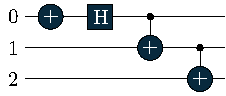
\includegraphics[width=0.3\textwidth]{src/ghz_circuit.pdf}. 
% \end{align}
% Instead of the \textsc{hadamard} we can also use a parametrized operation like $R_y(\theta)$
% \begin{align}
%     U = \textsc{cnot}(1,2)\textsc{cnot}(0,1)R_y(0,\theta)\textsc{not}(0)
% \end{align}
% the circuit representation of this operation looks basically the same. Here, we will sometimes color the parametrized gates to indicate that the parameter $\theta$ is not determined yet
% \begin{align}
%     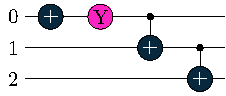
\includegraphics[width=0.3\textwidth]{src/ghz_ry_circuit.pdf}.
% \end{align}
% As a last example, we look at the circuit with the two \textsc{cnot} operations replaced by
% \begin{align}
%     R_{xy}(\theta) = e^{-i\frac{\theta}{2} X\otimes Y}  
% \end{align}
% with parametrization $\theta=\varphi$ (so a different parameter than in the $R_y$ rotation before) for the first and $\theta=\pi/2$ for the second gate. The final assembled unitary is then 
% \begin{align}
%     U = R_{xy}(\pi/2,1,2)R_{xy}(\varphi,0,1)R_y(0,\theta)\textsc{not}(0)
% \end{align}
% and the circuit is graphically depicted as
% \begin{align}
%     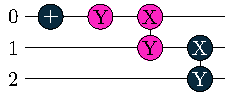
\includegraphics[width=0.3\textwidth]{src/ghz_xy_circuit.pdf},\label{eq:circuit_example_xy}
% \end{align}
% so the fact that the two parametrized gates carry individual parameters is often not emphasized (styles vary though). One can for example often see the explicit notation
% \begin{align}
%     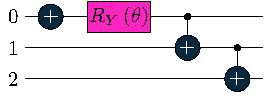
\includegraphics[width=0.3\textwidth]{src/alt_ghz_ry_circuit.pdf}.
% \end{align}

% General remarks:
% \begin{itemize}
%     \item gates that ``touch'' different qubits commute and can be executed in parallel (sometimes the collection of in-parallel executable gates is referred to as ``moments'')
%     \item runtime correlates with ``depth'' of the circuit (the number of moments in the circuit)
%     \item not all architectures are necessarily able to execute gates in parallel
% \end{itemize}
% The circuits shown so far all had depths 4 and all gates formed independent moments. Depending on what we are considering a primitive gate, these depths can however change. If only single-qubit Pauli rotations and \textsc{cnot}s are considered primitive operations, the $XY$ rotations from circuit~\eqref{eq:circuit_example_xy} need to be decomposed into sequences of those operations. In this chapter we will see how we can do this through a general framework generated by Pauli matrices.
